\documentclass[a4paper,12pt]{article} % Тип документа

\usepackage{graphicx}
\graphicspath{{pictures/}}
\DeclareGraphicsExtensions{.pdf,.png,.jpg}

% Русский язык
\usepackage[T2A]{fontenc}
\usepackage[utf8]{inputenc}
\usepackage[english,russian]{babel}

% Математика
\usepackage{amsmath,amsfonts,amssymb,amsthm,mathtools} 


\usepackage{wasysym}

%Заговолок
\author{Маллаев Руслан}
\title{Лабораторная работа №1.1.6}
\date{12 октября 2020 г.}

\begin{document} % Начало документа

\maketitle
\newpage

\textbf{Цель работы:} ознакомиться с утройством осциллографа и изучить

его основные характеристики.\\

\textbf{Приборы, используемые в работе:} осциллограф, генератор элек-

трических импульсов, соединительные кабели.
\newpage




\section{Измерение амплитуды синусоидального сигнала}
\[U_{max} = 10\text{ В}, U_{min} = 60\text{ мВ}\]\\
\[\beta = 20log\frac{U_{max}}{U_{min}} = 44.44\text{ дБ}\]




\section{Измерение частоты синусоидального сигнала}
\[\text{Таблица №1}\]
\begin{tabular}[h]{|c|c|c|c|c|c|c|}
\hline
$f_{\text{зг}}\text{, Гц}$   & $\frac{\text{ВРЕМЯ}}{\text{ДЕЛ}}$ & Т, ДЕЛ & Т, мс  & $f_{\text{изм}}\text{, Гц}$  & $|f_{\text{зг}} - f_{\text{изм}}|\text{, Гц}$ & $\frac{|f_{\text{зг}} - f_{\text{изм}}|}{f_{\text{зг}}}$ \\ \hline
1500  & 0.1мс/дел & 6.6   & 0.660 & 1515  & 15       & 0.010    \\ \hline
500   & 0.2мс/дел & 9.8   & 1.960 & 510   & 10       & 0.020    \\ \hline
100   & 1мс/дел   & 9.8   & 9.800 & 102   & 2        & 0.020    \\ \hline
10000 & 10мкс/дел & 9.8   & 0.098 & 10204 & 204      & 0.020    \\ \hline
15000 & 10мкс/дел & 6.7   & 0.067 & 14925 & 75       & 0.005    \\ \hline
\end{tabular}




\section{Влияние АЧХ на искажение сигнала}
$1)AC$\\
$\bullet\text{ } 50 \text{ и }100\text{ Гц}$
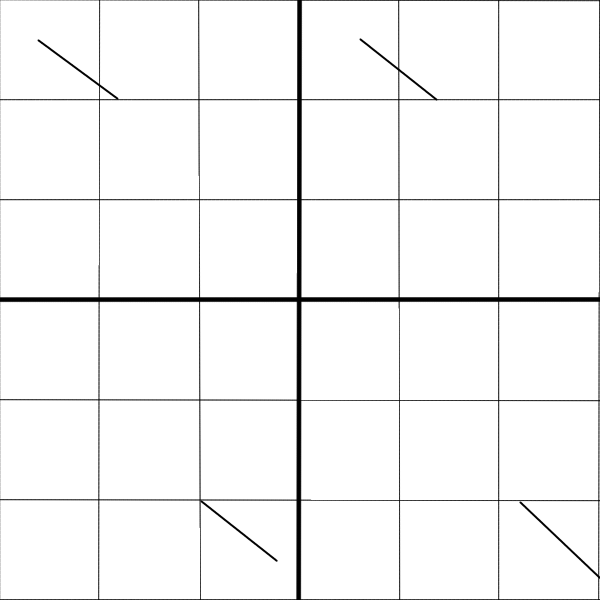
\includegraphics[scale=0.28]{100,50}
$\text{   }\bullet\text{ } 500\text{ Гц}$
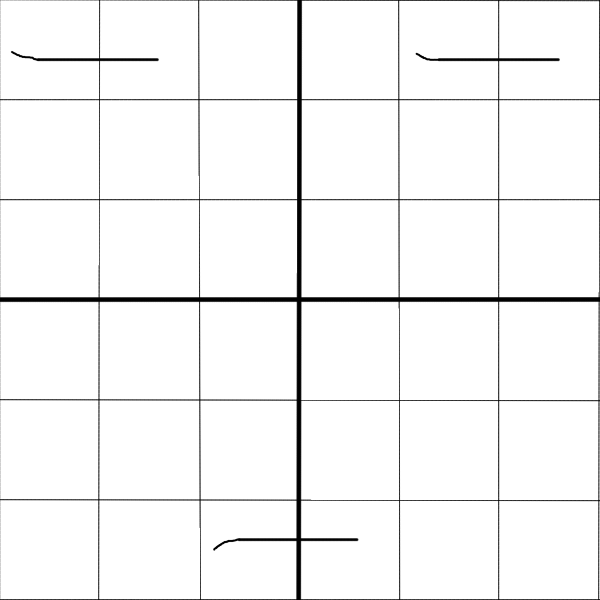
\includegraphics[scale=0.28]{500}\\
$\bullet\text{ } 1000\text{ Гц}\text{ }\text{ }\text{ }\text{ }$
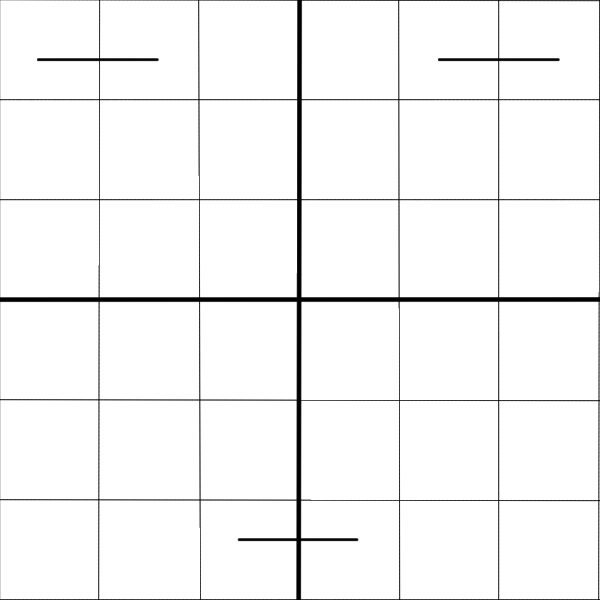
\includegraphics[scale=0.28]{1000}
$\text{   }\bullet\text{ } 10\text{ кГц}$
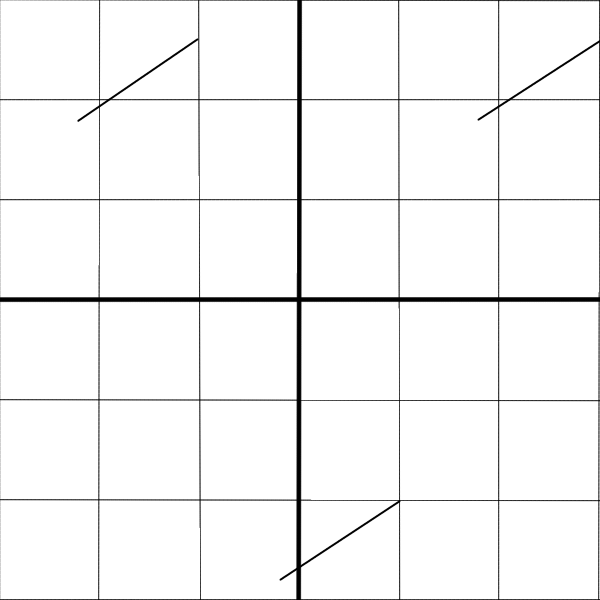
\includegraphics[scale=0.28]{10000}\\\\
$\bullet\text{ } 1\text{ МГц }\text{ }\text{ }\text{ }\text{ }\text{ }$
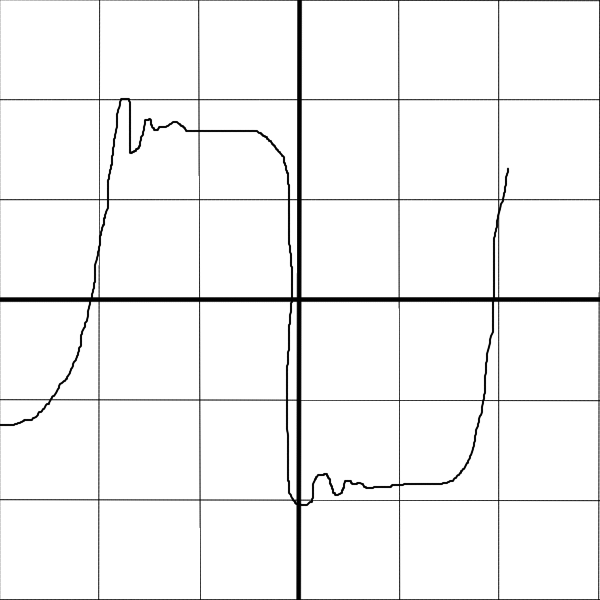
\includegraphics[scale=0.28]{1000000}\\\\
$2)DC$\\
$\bullet\text{ } 1 - 500\text{ Гц }$
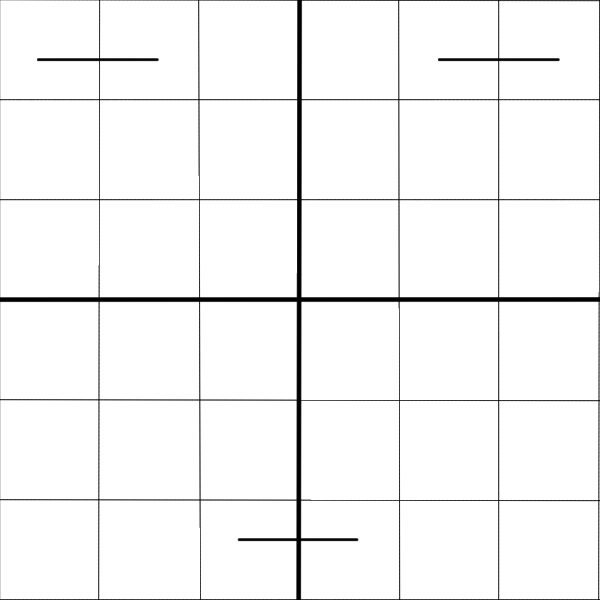
\includegraphics[scale=0.28]{1000}
$\bullet\text{ } 1000\text{ Гц}$
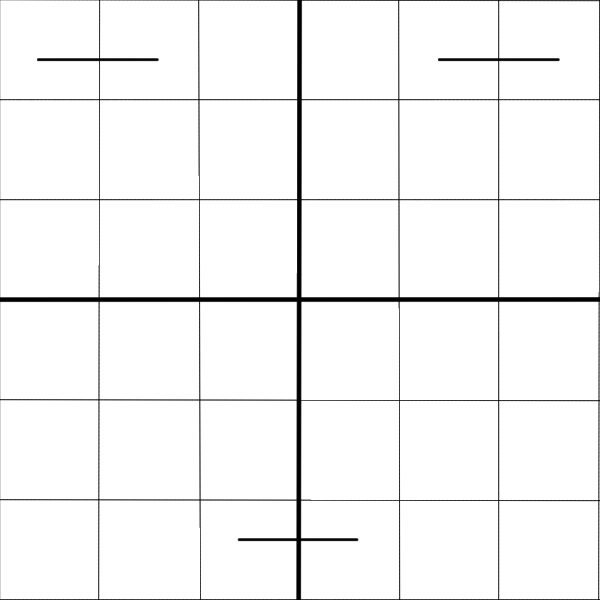
\includegraphics[scale=0.28]{1000}\\\\
$\text{   }\bullet\text{ } 10\text{ кГц}\text{ }\text{ }\text{ }\text{ }$
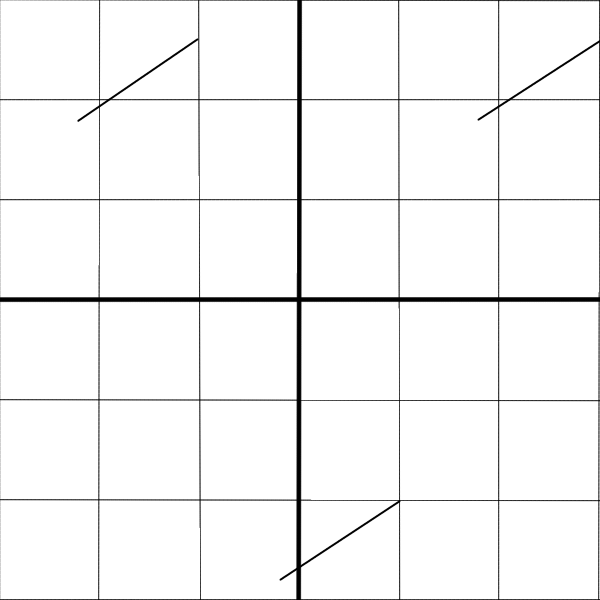
\includegraphics[scale=0.28]{10000}
$\bullet\text{ } 1\text{ МГц }\text{ }\text{ }$
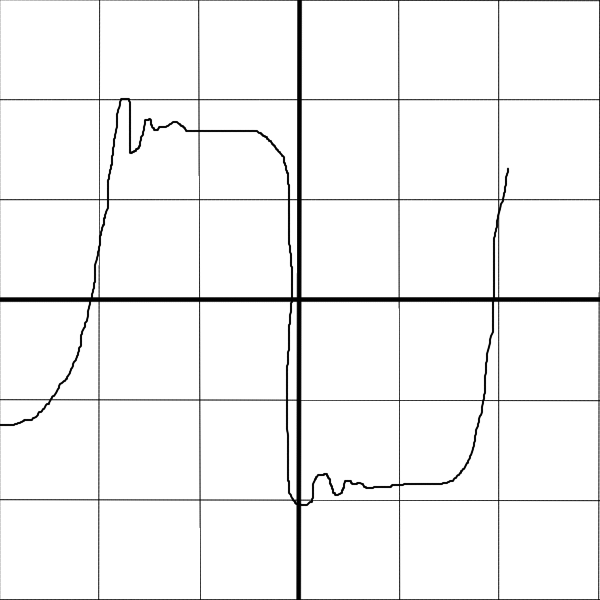
\includegraphics[scale=0.28]{1000000}\\




\section{Измерение разности фазовых сдвигов сигналов на выходах усилителей канала <<X>> и канала <<Y>> при одновременной подаче на их входы одного и того же сигнала, т.е. разности фазово-частотных характеристик каналов <<X>> и <<Y>>}
\begin{center}
\[\text{Таблица №2}\]
\begin{tabular}[h]{|l|c|c|c|c|c|c|c|}
\hline
$f_{\text{зг}}\text{, кГц}$           & 1     & 100   & 200   & 300   & 500   & 1000  & 1500  \\ \hline
A,дел           & 3     & 3     & 3     & 3     & 3     & 3     & 3     \\ \hline
B, дел           & 0.0     & 0.2   & 0.3   & 0.5   & 0.8   & 1.6   & 2.3   \\ \hline
$\bigtriangleup\Phi_{xy}$ & 0.00     & 0.067 & 0.100   & 0.167 & 0.270  & 0.563 & 0.874 \\ \hline
\multicolumn{8}{|l|}{}                                              \\ \hline
$f_{\text{зг}}\text{, кГц}$           & 2000  & 2120  & 2500  & 3000  & 3500  & 4000  & -     \\ \hline
A, дел           & 3     & 3     & 3     & 3     & 3     & 3     & -     \\ \hline
B, дел           & 2.8   & 3.0     & 2.7   & 1.8   & 0.7   & 0.1   & -     \\ \hline
$\bigtriangleup\Phi_{xy}$          & 1.204 & 1.571 & 2.022 & 2.498 & 2.906 & 3.108 & -     \\ \hline
\end{tabular}
\end{center}
При $f_{\text{зг}}$ менее 2.12 МГц эллипс наклонен влево, а при больших частотах вправо. При низких $f_{\text{зг}}$ не измеряется.\\
Построим график зависимости ln($\bigtriangleup\Phi_{xy}$) от ln($f_{\text{зг}}$)
\[\text{График №1}\]
\begin{center}
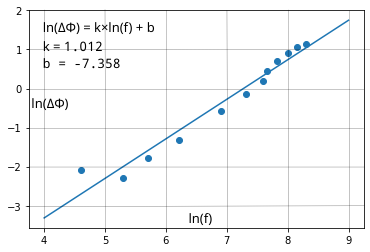
\includegraphics[scale=0.75]{fig}
\end{center}
Из графика можно сделать вывод, что $\bigtriangleup\Phi_{xy} = \alpha \cdot f_{\text{зг}}^{\beta}$, где $ln(\alpha) = b\text{; } \beta = k$



\section{Наблюдение фигур Лиссажу при сложении колебаний во взаимно перпендикулярных направлениях}
$\bullet \text{ }1:1$\\\\\\\\\newline
\begin{center}
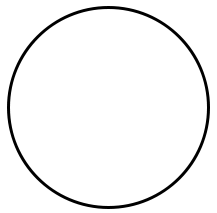
\includegraphics{11}
\end{center}
$\bullet \text{ }2:1$\\\\\\\\\newline
\begin{center}
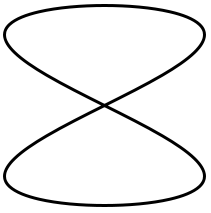
\includegraphics{12}
\end{center}
$\bullet \text{ }3:1$\\\\\\\\\newline
\begin{center}
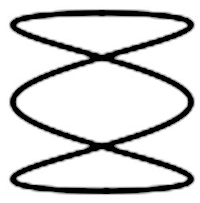
\includegraphics[scale=3.6]{13}
\end{center}
$\bullet \text{ }3:2$\\\\\\\\\newline
\begin{center}
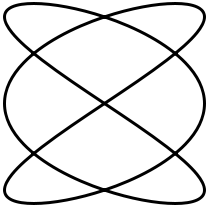
\includegraphics{23}
\end{center}
\end{document} % Конец документа